test-to-test\subsection{\Encode: Transcription factor binding across different cell types}
\label{sec:app_encode}

Here we provide details on the transcription factor binding dataset discussed in \refsec{genomics}.
Transcription factors (TFs) are regulatory proteins that bind specific DNA elements in the genome to activate or repress transcription of target genes.
There are estimated to be approximately 1,600 human TFs, and the binding landscape of each TF can be highly variable across different cell types \citep{deplancke16TFbindingreview}.
Understanding how these binding patterns change across different cell types and affect cellular function is critical for understanding the mechanics of dynamic gene regulation across cell types and across healthy and diseased cell states.

Several experimental strategies have been developed to profile genome-wide binding landscapes of individual TFs in specific cell types of interest.
However, genome-wide profiling of TF binding is challenging in practice, as it requires large numbers of cells and reagents (e.g., high-affinity antibodies) that are difficult and expensive to acquire.
Moreover, profiling each individual TF requires a separate experiment, so it can be prohibitively costly to map out even a few different TFs out of the \textgreater 1000 in the human genome.
Therefore, there has been wide interest in computational approaches that can predict the genome-wide binding maps of multiple TFs in new cell types from a single and more practical genome-wide assay.

DNA sequence is one of the principal determinants of where a TF binds along the genome,\footnote{Most TFs, including the ones we provide in this benchmark, have DNA-binding domains which bind to sequence motifs: short recognition sequences (4-20 bases in length) in the genome with specific binding affinity distributions \citep{StormoZ10}.}
and many ML models have been developed to predict TF binding as a function of DNA sequence in a particular cell type \citep{deepbind15, quang2019factornet, avsec2021base}.
However, even when the DNA sequence is invariant across different cell types (e.g., among cell types from the same organism), the TF binding landscape can still be highly variable \citep{deplancke16TFbindingreview}.
Therefore, TF binding models that only use sequence inputs cannot make different predictions for the same sequence across different cell types;
we also need complementary, cell-type-specific inputs to model changes in binding over different cell types.

In this section, we explore the use of genome-wide chromatin accessibility assays such as DNase-seq and ATAC-seq \citep{boyle2008high, DNaseLandscape12, ATAC13}, in conjunction with DNA sequence, to predict TF binding.
DNA is typically accessible in a highly local and cell-type-specific manner,
and in particular, genomic sequences with high accessibility are typically bound by one or more TFs, although the identity of the TF is not directly measured by the experiment \citep{lee2004evidence}.
By measuring chromatin accessibility at each base in the genome in a specific cell type of interest, we can obtain a cell-type-specific profile of binding locations; moreover, these experiments are often cheaper than profiling even a single TF \citep{minnoye2021chromatin}.
Our goal is to use this accessibility signal, combined with DNA sequence, to accurately predict the binding patterns of multiple TFs in new cell types.

We study the problem of predicting genome-wide TF binding across different cell types using data from the ENCODE-DREAM Transcription Factor Binding Site Prediction Challenge \citep{EDsynapse}.


\subsubsection{Setup}
\paragraph{Problem setting.}
We consider the domain generalization setting, where the domains are cell types, and we seek to learn models that can generalize to cell types that are not in the training set.
The task is to predict if a particular transcription factor (TF) would bind to a particular genomic location in a cell type of interest (\reffig{etwilds-schematic}).
The input is DNA sequence (which we assume to be shared across all cell types) and a cell-type-specific biochemical measurement of chromatin accessibility obtained through the DNase-seq assay.

Concretely, we segment the genome into uniformly-sized, overlapping bins that are 200 base pairs (bp) in length, and tiled 50bp apart. Given a TF $p$, each genomic bin $i$ in cell type $d$ has a binding status $y^{p}_{i, d} \in \{0, 1\}$.
Our goal is to predict each bin's binding status as a function of the local DNA sequence $S_i$ and the local cell-type specific accessibility profile $A_{i,d}$ (\reffig{etwilds-schematic}). We treat each TF separately, i.e., for each $p$, we have separate training and test sets and separate models.

For computational convenience, we consider input examples $x \in \R^{12800 \times 5}$ that each represent a window of 12800 bp and span several genomic bins. The first four columns of $x$ is a binary matrix representing a one-hot encoding of the four bases (A,C,G,T) of the DNA sequence at that base pair. The 5th column is a real-valued vector representing chromatin accessibility.
We tile the central 6400 bp of the window with 128 overlapping bins of length 200 bp, tiled 50 bp apart.\footnote{This ensures that each bin has at least 3200 bp of context on either side of it for prediction.}
Thus, each $x$ is associated with a target output $y \in \{-1,0,1\}^{128}$ indicating the binding status of the TF at each of these 128 bins. The three possible values at each bin indicate whether the bin is bound, unbound, or ambiguous.
During training and testing, we simply ignore ambiguous bins, and only focus on bound or unbound bins.
The domain $d$ is an integer that identifies the cell type.


\begin{figure*}[h]
\begin{center}
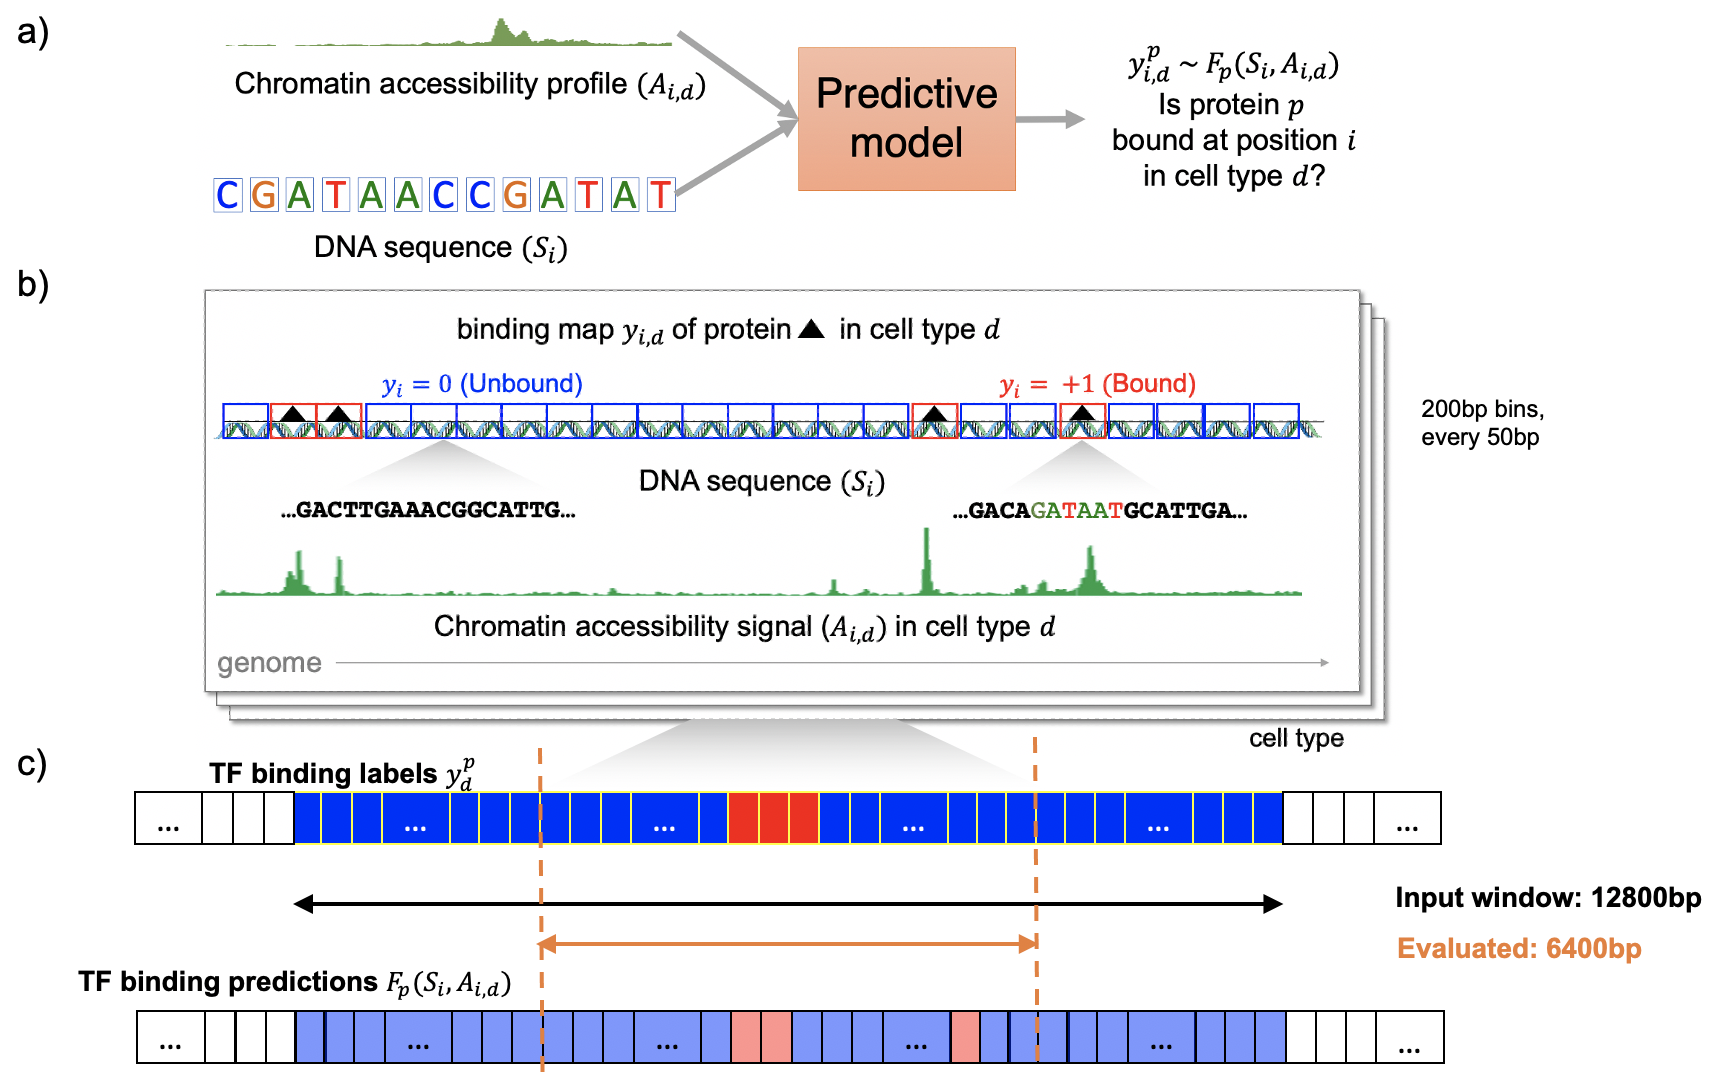
\includegraphics[width=\textwidth]{figures/Wilds_ENCODE-DREAM-schematic.png}
\end{center}
\caption{
Setup of the \Encode benchmark. (a) The predictive model predicts binding of a protein to a location, in a cell type (domain). (b) The input features are DNA sequence and chromatin accessibility, and the labels are assigned over 200 base pair (bp) bins tiling the genome every 50 bp. (c) Each training example is a 12800 bp window, with the 128 middle bins evaluated (spanning 6400 bp).
}
\label{fig:etwilds-schematic}
\end{figure*}


\paragraph{Data.}
The dataset comprises (a) genome-wide sequence; (b) TF binding maps for two TFs, JUND and MAX, across a total of 6 and 8 cell types respectively; and (c) an accessibility profile for each cell type.
As described above and illustrated in \reffig{etwilds-schematic}, we break up these genome-wide data into overlapping 12800 bp windows, which each correspond to a single training example.
The central 6400 bp of each 12800 bp window is tiled with overlapping 200 bp bins that each correspond to one coordinate of the corresponding $y \in \{0,1\}^{128}$.
These 12800 bp windows are tiled 6400 bp apart, such that each genomic location falls within the central 6400 bp region of exactly one window.

We split the examples by domain (cell type) as well as by chromosome (a large contiguous subsequence of the genome) within a cell type.
In each split, we use one cell type for the test data, one for the validation data, and the remaining cell types for the training data.
These domain-wise splits are listed in \reftab{splits}, and are divided into two types:
\begin{enumerate}
  \item The \emph{ENCODE-DREAM} splits follow the original challenge setup \citep{EDsynapse} closely in evaluating only on the cell type \texttt{liver}, which is a primary tissue, in contrast to all of the other cell types, which are immortalized cell lines that have been grown outside the body for many generations. This is a more realistic setting in the sense that it is easier to collect data from immortalized cell lines, which we can then use to train a model that predicts TF binding in harder-to-profile primary tissues.
  However, the fact that none of the training cell types are primary tissues might limit generalization to primary tissues. Moreover, because cell types are highly variable, conclusions drawn from a single \texttt{liver} cell type might not generalize to other cell types.
  \item We thus also use a \emph{round-robin} set of splits, where we assign each cell type to test and validation sets in a rotating manner. This round-robin evaluation comprises several splits for each TF.
\end{enumerate}

For each split in \reftab{splits}, the data are divided into training, validation, and test sets by chromosome:
\begin{enumerate}
    \item
    \textbf{Training: }
    323,894 windows per training cell type, before filtering.  To improve class balance, we filter out windows with all 128 bins labeled negative, which typically removes over 3/4 of these training windows; the exact number filtered out depends on the split.
    The training windows are taken from all chromosomes except $\{ 1, 2, 8, 9, 11, 21 \}$.
    \item
    \textbf{Validation (OOD): }
    27,051 windows from 1 validation cell type and from chromosomes $\{ 2, 9, 11 \}$.
    \item
    \textbf{Test (OOD): }
    23,109 windows from 1 test cell type and from chromosomes $\{ 1, 8, 21 \}$.
    \item
    \textbf{Validation (ID): }
    27,051 windows in total across all training cell types, from chromosomes $\{ 2, 9, 11 \}$.
    \item
    \textbf{Test (ID): }
    23,109 windows in total across all training cell types, from chromosomes $\{ 1, 8, 21 \}$.
\end{enumerate}

For computational speed, the Validation (OOD) and Test (OOD) sets above were subsampled by a factor of 3 from the available raw data, while the Validation (ID) and Test (ID) sets were subsampled by a factor of 3 $\times$ the number of training cell types.


\begin{table*}[t]
  \caption{
  List of splits for which we trained models for \Encode.
  Performance of models on round-robin splits are averaged to get the summarized results in \reftab{results_roundrobin}.
  }
  \label{tab:splits}
  \begin{center}
  \begin{small}
  \begin{tabular}{cccc}
  \toprule
  Split name & TF name & Test cell type & Validation cell type  \\
  \midrule
  ENCODE-DREAM & MAX & liver &  HepG2  \\
  \midrule
  round-robin & MAX & K562  & liver  \\
  round-robin & MAX & liver & A549     \\
  round-robin & MAX & A549  & GM12878   \\
  round-robin & MAX & GM12878 &  H1-hESC  \\
  round-robin & MAX & H1-hESC  & HCT116  \\
  round-robin & MAX & HCT116  & HeLa-S3  \\
  round-robin & MAX & HeLa-S3 &  HepG2  \\
  round-robin & MAX & HepG2  & K562 \\
  \midrule
  ENCODE-DREAM & JUND & liver &  HepG2  \\
  \midrule
  round-robin & JUND & K562 &  liver  \\
  round-robin & JUND & liver &  MCF-7   \\
  round-robin & JUND & MCF-7 & HCT116  \\
  round-robin & JUND & HCT116  & HeLa-S3   \\
  round-robin & JUND & HeLa-S3  & HepG2  \\
  round-robin & JUND & HepG2  & K562  \\
  \bottomrule
  \end{tabular}
  \end{small}
  \end{center}
  \vspace{-4mm}
\end{table*}


\paragraph{Evaluation.}
We evaluate models by their average precision (AP) in predicting binary binding status (excluding all ambiguous bins). Specifically, we treat each bin as a separate binary classification problem; in other words, we split up each prediction of the 128-dimensional vector $y$ into at most 128 separate binary predictions after excluding ambiguous bins. We then compute the average precision of the model on this binary classification problem.

The choice of average precision as an evaluation metric is motivated by the class imbalance (low proportion of bound/positive labels) of this binary classification problem over bins.
All splits have more than one hundred times as many unbound bins than bound bins (\reftab{label_imbalance}).



\begin{table*}[t]
  \caption{Binding site imbalance and uniqueness (across cell types) in binary genome-wide binding datasets in \Encode.
  Third column indicates the fraction of (non-ambiguous) bins that are labeled positive.
  Fourth column indicates the fraction of positive bins (bound sites) that are cell-type-specific: they are bound (or ambiguous) in at most one other cell type.
  Bins are 200bp wide.
  }
  \label{tab:label_imbalance}
  \begin{center}
  \begin{small}
  \begin{tabular}{cccc}
  \toprule
  TF name & Cell type &  Frac.~positive bins  &  Frac.~cell-type-specific binding sites \\
  \midrule
  MAX  &  liver  & $4.90 \times 10^{-3}$ &  0.518 \\
  MAX  &  HepG2  & $6.20 \times 10^{-3}$ &  0.331 \\
  MAX  &  K562  & $6.46 \times 10^{-3}$ &  0.368 \\
  MAX  &  A549  & $5.90 \times 10^{-3}$ &  0.218 \\
  MAX  &  GM12878  & $1.93 \times 10^{-3}$ &  0.217 \\
  MAX  &  H1-hESC  & $4.44 \times 10^{-3}$ &  0.363 \\
  MAX  &  HCT116  & $6.46 \times 10^{-3}$ &  0.237 \\
  MAX  &  HeLa-S3  & $4.21 \times 10^{-3}$ &  0.218 \\
  \midrule
  JUND  &  liver  & $4.45 \times 10^{-3}$ &  0.523 \\
  JUND  &  K562  & $3.94 \times 10^{-3}$ &  0.408 \\
  JUND  &  HCT116  & $4.08 \times 10^{-3}$ &  0.297 \\
  JUND  &  HeLa-S3  &  $3.60 \times 10^{-3}$ &  0.323 \\
  JUND  &  HepG2  & $3.54 \times 10^{-3}$ &  0.513 \\
  JUND  &  MCF-7  &  $1.84 \times 10^{-3}$  &  0.335 \\
  \bottomrule
  \end{tabular}
  \end{small}
  \end{center}
  \vspace{-4mm}
\end{table*}


\subsubsection{Baseline results}

\paragraph{Model.}

Our model is a version of the fully convolutional U-Net model for image segmentation \citep{ronneberger2015u}, modified from the architecture in \cite{li2019leopard}. It is illustrated in \reffig{etwilds_arch}.
We train each model using the average cross-entropy loss over the 128 output bins in each example (after excluding ambiguous bins).

\begin{figure*}[h]
\begin{center}
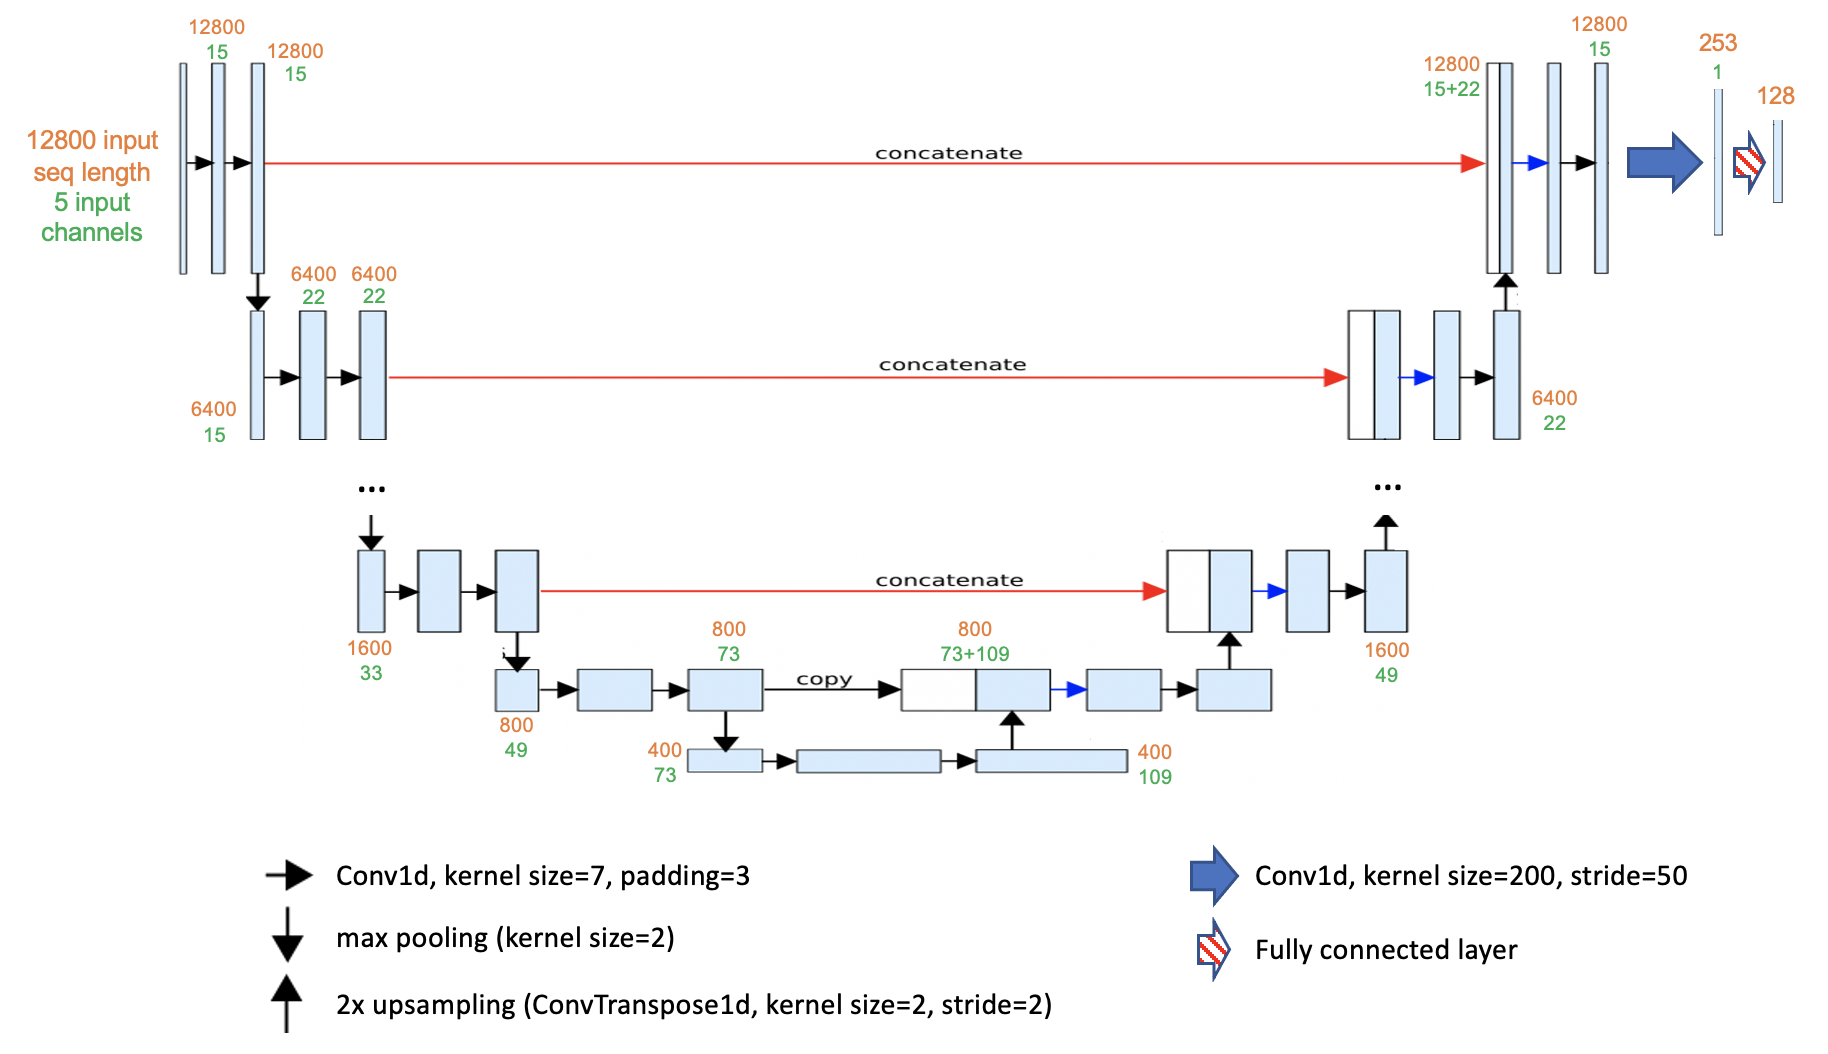
\includegraphics[width=\linewidth]{figures/Unet-seq-wilds.png}
\end{center}
\caption{
    Architecture of the baseline prediction model, based on U-Net.
    The final layers were modified to collapse the representation down to a single channel and finally convolved with kernel size 200 and stride 50, mimicking the resolution of labels along the genome.
}
\label{fig:etwilds_arch}
\end{figure*}

For hyperparameters, we searched over the learning rates $\{ 10^{-5}, 10^{-4}, 10^{-3} \}$, and $L_2$-regularization strengths $\{ 10^{-4}, 10^{-3}, 10^{-2} \}$.
We use 10 replicates (with different random seeds) for all reported results.


\paragraph{ERM results.}

\reftab{results_roundrobin} and \reftab{results_ood_full} show the results of ERM models trained on each split.
On many individual splits (\reftab{results_ood_full}), the OOD validation and OOD test performance are very different, reflecting the variability across the cell types.
On average across the round robin splits, the OOD validation performance is slightly higher than the OOD test performance, as we selected hyperparameters and did early stopping to maximize the former (\reftab{results_roundrobin}).
We also observed high variance in training and test performance across random seeds in a few splits (e.g., the K562 / liver split for the transcription factor JUND), which suggests some optimization instability in our training protocol.
We also computed the in-distribution baselines in a train-to-train setting, i.e., on the Validation (ID) and Test (ID) splits described above.

We also ran corresponding in-distribution baselines in a test-to-test setting, i.e., we trained ERM models on data from the training chromosomes in the test cell type, and tested it on the same test set comprising data from the test chromosomes in the test cell type.\footnote{
Prior work has shown that there is minimal variation in performance between chromosomes on this problem \citep{won2010genome, deepbind15, keilwagen2019accurate}, so we can approximate these training and test distributions as identical.
}
\reftab{results_etwilds_id} shows these in-distribution results.
For the round-robin splits, the difference between the train-to-train and test-to-test settings is that the former trains and tests on mixtures of multiple cell types, whereas the latter trains and tests on individual cell types.

We considered two TFs, MAX and JUND, separately.
For the ENCODE-DREAM splits, both TFs showed large ID-OOD performance gaps.
However, we opted not to use the ENCODE-DREAM split as a \Wilds dataset
because the variability between cell types made us cautious about over-interpreting the results on a single cell type. For example, for MAX, we found that the Validation (OOD) and Test (OOD) cell types were so different that their results were anti-correlated across different random seeds, which would have made benchmarking challenging.
Moreover, the fact that the test cell type (\texttt{liver}) in the ENCODE-DREAM splits was the only primary tissue might have meant that the training data might have insufficient leverage for a model to learn to close the ID-OOD gap.

We therefore focused on analyzing the round-robin splits.
For MAX, using the train-to-train comparison, the average Test (ID) and Test (OOD) AP across the round-robin splits were not significantly different (64.9 (2.1) vs.~59.6 (2.0), respectively; \reftab{results_roundrobin}).
For JUND, using the train-to-train comparison, the average Test (ID) and Test (OOD) AP across the round-robin splits showed a larger gap (54.1 (4.2) vs.~42.9 (3.2), respectively; \reftab{results_roundrobin}), but the variability in training performance made these results less reliable. Moreover, the test-to-test ID results were significantly higher than the train-to-train ID results (62.4 (2.6) vs.~54.1 (4.2), respectively), which suggests that either the model capacity or feature set is not rich enough to fit the variation across different cell types.
We therefore opted not to include the round-robin splits in \Wilds as well.

\begin{table*}[t]
  \caption{ERM baseline results on \Encode.
  All numbers are average precision.
  ``Round-robin'' indicates the average performance over all splits marked ``round-robin'' in \reftab{splits}.
  Parentheses show standard deviation across replicates, for \texttt{liver}; and average of such standard deviations across splits, for \texttt{round-robin}.
  Expanded results per round-robin split are in \reftab{results_id_full}.
  }
  \label{tab:results_roundrobin}
  \begin{center}
  \begin{small}
  \begin{tabular}{lccccc}
  \toprule
  TF & Split scheme & Validation (ID) & Test (ID) & Validation (OOD) & Test (OOD) \\
  \midrule
  MAX &  ENCODE-DREAM  &   70.3 (2.1)  &   68.3 (1.9) & 67.9 (1.6) & 45.0 (1.5)   \\
  MAX &  round-robin  &  65.0 (2.1)  & 64.9 (2.1)  & 62.1 (1.2)  & 59.6 (2.0) \\
  \midrule
  JUND &  ENCODE-DREAM  &   65.9 (1.2)  &  66.7 (1.4)  & 32.9 (1.0) & 42.3 (2.5) \\
  JUND &  round-robin  & 53.2 (4.0)  & 54.1 (4.2)  & 47.2 (2.4)  & 42.9 (3.2)  \\
  \bottomrule
  \end{tabular}
  \end{small}
  \end{center}
  \vspace{-4mm}
\end{table*}


\begin{table*}[t]
  \caption{In-distribution results on \Encode: when training and validation cell types are set to the test cell type.
  All numbers are average precision.
  ``Round-robin'' indicates the average performance over all splits marked ``round-robin'' in \reftab{splits}.
  Parentheses show standard deviation across replicates, for \texttt{liver}; and average of such standard deviations across splits, for \texttt{round-robin}.
  Expanded results per round-robin split are in \reftab{results_id_full}.
  }
  \label{tab:results_etwilds_id}
  \begin{center}
  \begin{small}
  \begin{tabular}{lcccc}
  \toprule
  TF & Split scheme & Train & Validation (ID) & Test (ID) \\
  \midrule
  MAX &  ENCODE-DREAM  & 76.1 (0.9)  &  57.3 (1.2)  &  57.6 (1.3)  \\
  MAX &  round-robin  &  77.3 (0.9)  &  65.2 (1.3)  &  65.4 (1.3)  \\
  \midrule
  JUND &  ENCODE-DREAM  &   76.0 (0.6)  &  55.8 (0.5)  &  56.0 (0.7) \\
  JUND &  round-robin  &  79.3 (2.7)  &  61.8 (2.4)  &  62.4 (2.6)  \\
  \bottomrule
  \end{tabular}
  \end{small}
  \end{center}
  \vspace{-4mm}
\end{table*}

\begin{table}[t]
  \caption{Baseline results on \Encode.
  In-distribution (ID) results correspond to the train-to-train setting.
  Parentheses show standard deviation across replicates.
  }
  \label{tab:results_ood_full}
  \begin{center}
  \begin{small}
  \resizebox{\textwidth}{!}{
  \begin{tabular}{lcccccc}
  \toprule
  TF name  & Test / Val cell type & Train AP & Val (ID) AP & Test (ID) AP & Val (OOD) AP & Test (OOD) AP \\
  \midrule \midrule
  MAX  & liver / HepG2  &  79.5 (1.0)  &   70.3 (2.1)  &   68.3 (1.9) & 67.9 (1.6) & 45.0 (1.5) \\
  \midrule
  MAX  & K562 / liver &  75.1 (2.3)  &   59.9 (4.5)  &   59.2 (3.9) & 47.6 (1.0) & 63.6 (4.5) \\
  MAX  & liver / A549  &  78.5 (1.3)  &   68.6 (0.8)  &   68.4 (0.5) & 66.6 (1.3) & 38.5 (1.1) \\
  MAX  & A549 / GM12878 &  78.0 (1.7) &  66.0 (2.6)  &  66.6 (2.8) &  46.9 (1.9)  & 65.0 (2.5)  \\
  MAX  & GM12878 / H1-hESC  &  80.0 (1.2)  &  69.6 (0.8)  &  69.2 (0.6) & 65.4 (0.7) & 46.3 (0.5) \\
  MAX  & H1-hESC / HCT116  &  75.5 (3.3)  &   63.2 (3.2)  &   63.9 (3.3) & 70.6 (0.5) & 61.7 (2.5) \\
  MAX  & HCT116 / HeLa-S3 &  76.8 (1.1)  &   64.5 (1.6)  &   64.9 (1.3) & 63.9 (0.9) & 69.4 (0.9) \\
  MAX  & HeLa-S3 / HepG2 &  77.7 (1.7)  &   65.0 (1.9)  &   64.8 (3.3) & 67.7 (1.9) & 64.0 (2.5) \\
  MAX  & HepG2 / K562 &  77.3 (1.3)  &   63.2 (1.3)  &   62.1 (1.4) & 68.5 (1.1) & 68.4 (1.1) \\
  \midrule \midrule
  JUND  & liver / HepG2  & 82.6 (1.3)  &   65.9 (1.2)  &   66.7 (1.4)  & 32.9 (1.0) & 42.3 (2.5)  \\
  \midrule
  JUND  & K562 / liver  &  54.2 (10.5)  &   29.9 (8.4)  &   33.3 (8.4)  & 32.9 (3.7) & 51.2 (4.5)  \\
  JUND  & liver / MCF-7  & 83.6 (2.4)  &   65.5 (3.4)  &   65.3 (4.0)  & 28.9 (2.7) & 29.2 (3.2) \\
  JUND  & MCF-7 / HCT116 &  76.4 (3.5)  &   52.5 (3.4)  &   53.6 (3.8)  & 51.8 (3.7) & 27.2 (4.2) \\
  JUND  & HCT116 / HeLa-S3  &  75.7 (1.5)  &   50.0 (2.4)  &   50.6 (2.4)  & 69.2 (2.1) & 52.9 (3.2) \\
  JUND  & HeLa-S3 / HepG2 &  78.0 (2.1)  &   59.5 (5.1)  &   60.0 (4.9)  & 30.3 (1.3) & 66.6 (3.6) \\
  JUND  & HepG2 / K562 &  79.6 (0.9)  &   61.9 (1.1)  &   62.3 (1.4)  & 69.8 (0.6) & 30.5 (0.6) \\
  \bottomrule
  \end{tabular}
  }
  \end{small}
  \end{center}
  \vspace{-4mm}
\end{table}

\begin{table}[t]
  \caption{Test-to-test results on \Encode.
  Parentheses show standard deviation across replicates.
  }
  \label{tab:results_id_full}
  \begin{center}
  \begin{small}
  \begin{tabular}{lcccc}
  \toprule
  TF name  & Test cell type & Train & Val (ID) AP & Test (ID) AP\\
  \midrule \midrule
  MAX  & liver  & 76.1 (0.9)  &  57.3 (1.2)  &  57.6 (1.3) \\
  \midrule
  MAX  & HepG2  & 76.1 (0.8)  &  66.5 (1.1)  &  68.4 (1.3) \\
  MAX  & K562  & 83.6 (0.7)  &  74.7 (0.8)  &  75.9 (0.7)  \\
  MAX  & A549  &  77.2 (0.8)  &  68.4 (1.4)  &  67.5 (1.5)  \\
  MAX  & GM12878  &  64.7 (0.8)  &  50.9 (1.3)  &  49.2 (1.5)  \\
  MAX  & H1-hESC  &  76.2 (1.8)  &  65.3 (2.1)  &  64.1 (1.9) \\
  MAX  & HCT116  &  82.8 (0.7)  &  73.6 (0.8)  &  74.5 (0.8)  \\
  MAX  & HeLa-S3  &  80.5 (0.8)  &  64.8 (1.4)  &  66.4 (1.4)  \\
  \midrule \midrule
  JUND  & liver  &  76.0 (0.6)  &  55.8 (0.5)  &  56.0 (0.7) \\
  \midrule
  JUND  & K562  & 87.3 (1.3)  &  74.5 (1.1)  &  76.0 (1.7)  \\
  JUND  & HCT116  &  80.9 (2.8)  &  69.5 (4.9)  &  68.4 (4.7)  \\
  JUND  & HeLa-S3  &  87.2 (0.8)  &  69.0 (0.7)  &  70.9 (0.8) \\
  JUND  & HepG2  &  84.1 (9.8)  &  71.9 (4.6)  &  72.1 (4.9) \\
  JUND  & MCF-7  &  60.1 (0.8)  &  30.1 (2.4)  &  31.1 (2.9) \\
  \bottomrule
  \end{tabular}
  \end{small}
  \end{center}
  \vspace{-4mm}
\end{table}


\paragraph{Discussion.}
Even in the in-distribution (test-to-test) setting, the results in \reftab{results_id_full} show how
different model performance can be for different domains.
For example, the \texttt{liver} domain of primary tissue (from a human donor) is derived from lower-quality data than many of the long-standard cell lines (grown outside the human body) constituting other domains, and is consequently noisier than many of them \citep{EDneurips17}.
The extent of this variation underscores the importance of accounting for the variability between domains when measuring the effect of distribution shift;
for example, a train-to-train comparison could lead to significantly different conclusions than a test-to-test comparison.

The effect of the distribution shift also seems to depend on the particular TF (MAX vs.~ JUND) used.
Biologically, different TFs show different levels of cell-type-specificity, and better understanding which TFs have binding patterns that can be accurately predicted from the cell-type-specific accessibility assays is important future work.

One of the main obstacles preventing us from using this ENCODE dataset as a \Wilds benchmark is the instability in optimization that we reported above.
We speculate that this instability could, in part, be due to the class imbalance in the data, but more work will be needed to ascertain this and to develop methods for training models more reliably on this type of genomic data.

As we mentioned above, \reftab{results_roundrobin} reports significantly higher test-to-test ID results than train-to-train ID results for the JUND round-robin split scheme. The main difference between the test-to-test and train-to-train settings in the round-robin splits is that the former trains and tests on a single cell type, whereas the latter trains and tests on a mixture of cell types. The fact that ID performance is significantly higher in the former than the latter suggests that the learned models are not able to fit JUND binding patterns across multiple cell types.
This could be due to a model family that is not large or expressive enough, or it could be because the feature set does not have all of the necessary information to accurately predict binding across cell types.
In either case, it is unlikely that a training algorithm developed to be robust to distribution shifts will be able to significantly improve OOD performance in this setting, as the issue seems to lie in the model family or the data distribution instead.

Overall, it is commonly understood that distribution shifts between cell types are a significant problem for TF binding prediction, and many methods have been developed to tackle these shifts \citep{EDneurips17, li2019anchor, li2019leopard, keilwagen2019accurate, quang2019factornet}.
Nonetheless, we found it challenging to establish a rigorous distribution shift benchmark around this task,
as our results were confounded by factors such as optimization issues, large variability between cell types,
and the difficulty of learning a model that could fit multiple cell types even in an i.i.d. setting.
We hope that future work on evaluating and mitigating distribution shifts in TF binding prediction
can build upon our results and address these challenges.


\subsubsection{Additional details}
\label{sec:app_etwilds}

\paragraph{Additional dataset details.}
The ground-truth labels were derived from high-quality chromatin immunoprecipitation sequencing (ChIP-seq) experiments, which provide a genome-wide track of binding enrichment scores for each TF.
Statistical methods based on standardized pipelines \citep{EncodeChipseq12} were used to identify high-confidence binding events across the genome, resulting in a genome-wide track indicating whether each of the windows of sequence in the genome is bound or unbound by the TF, or whether binding is ambiguous but likely (these were ignored in our benchmarking).

Our data include two TFs chosen for their basic importance in cell-type-specific gene regulation: MAX and JUND.
MAX canonically recognizes a short, common sequence (the domain CACGTG), but its structure leads it to bind to DNA as a dimer, and facilitates cooperative activity with a range of partners \citep{grandori2000myc} with many weaker and longer-range sequence determinants of binding \citep{allevato2017sequence}.
JUND belongs to a large family of TFs (bZIP) known for binding in cooperation with partners in the family in a variety of modes, all involving a short 7bp sequence (TGA[C/G]TCA) and its two halves.

\paragraph{Additional model details.}

The network consists of encoder and decoder portions:
\begin{itemize}
\item
\textbf{Encoder. } The encoder is composed of five downscaling convolutional blocks, each consisting of two stride-1 convolutional layers with kernel size 7 (and padding such that the output size is left unchanged), followed by a max-pooling layer with kernel size 2.
Each successive block halves the input window size and scales up the number of convolutional filters (by 1.5).
\item
\textbf{Decoder. } Mirroring the encoder, the decoder is composed of five upscaling convolutional blocks, each consisting of two convolutional layers with kernel size 7 and an upsampling layer (a ConvTranspose layer with kernel size 2 and stride 2).
Each successive block doubles the input window size.
The respective sizes of the decoder layer representations are the same as the encoder in reverse, culminating in a $(12800 \times 15)$ representation that is then run through a convolutional layer (kernel size 200, stride 50) to reduce it to a single channel (with length 253).
A final fully-connected layer results in a 128-dimensional output.
\end{itemize}
Batch normalization is applied after every layer except the last, and each intermediate convolutional layer is padded such that the output and input sizes are equal.

\paragraph{Additional data sources.}
The ENCODE-DREAM prediction challenge contains binding data for many TFs from a large range of cell types,
discretized into the same 200-bp windows used in this benchmark.
The ENCODE portal (\texttt{encodeproject.org}) contains more ChIP-seq datasets from the 13 challenge cell lines for which we provide DNase accessibility data.
DNA shape and gene expression data types were also provided in the original challenge.
\begin{itemize}
\item
\textbf{DNA shape. } Twisting, bending, and shearing of DNA influence local binding in a TF-specific fashion \citep{RohsShape09}.
\item
\textbf{Gene expression. } Expression levels of all human genes were provided using RNA-seq data from ENCODE. This can be used to model the presence of cofactor proteins that can recruit TFs for binding \citep{PG97}.
\end{itemize}
However, none of the top challenge participants found these data modalities useful \citep{EDneurips17}, so they are not provided in this benchmark.



\paragraph{Data normalization. }

We normalize the distribution of each DNase-seq signal readout to the average of the DNase-seq signals over training cell types.
We use a version of quantile normalization \citep{bolstad2003comparison} with piecewise polynomial interpolation.
\cite{li2019leopard} also use this, but instead normalize to the test domain's DNase distribution.
As this technique uses test-domain data, it is out of the scope of our benchmark.
However, we note that in genomics settings it is realistic to have relatively cheaply available chromatin accessibility data in the target cell type of interest.

\paragraph{Modifications to the original setup. }
The prediction task of the challenge was a binary classification problem over the 200 bp bins, which did not involve the fixed 12800 bp windows.
To predict on a bin, participating teams were free to use as much of the regions surrounding (flanking) the bin as they wished.
The winning teams all used at least 1000 bp total for each bin, and further work has shown the efficacy of using much larger flanking regions of tens of thousands of bp \citep{quang2019factornet, enformer21}.
We instead predict on 128 bins at once (following \cite{li2019leopard}),
which allows for more efficient training and prediction.

Our ERM baselines' OOD test performance is competitive with the original challenge results, but lower than the state-of-the-art performance of \cite{li2019leopard} because of the aforementioned differences in data processing, splits, and architecture, as well as the cross-domain training method employed by that paper and predecessor work \citep{li2019anchor}.
These and other state-of-the-art models noted that their domain adaptation strategies played a major role in improving performance.
